\documentclass{article}
\usepackage{tikz}
\usepackage{adjustbox}

\begin{document}

\begin{center}
    {\ttfamily \textbf{Mission Display:}}
\end{center}

\begin{adjustbox}{center}
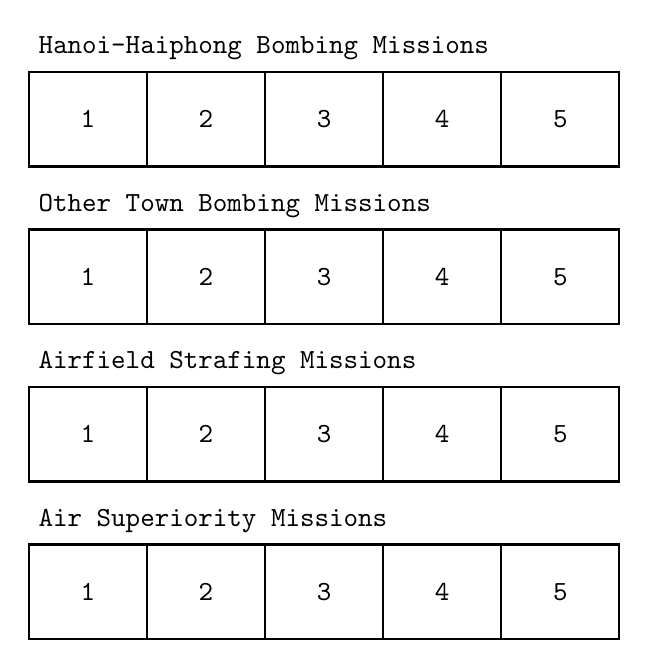
\begin{tikzpicture}
    % Define box size
    \def\boxwidth{1.5}
    \def\boxheight{1.2}

    % Define mission numbers
    \def\numbers{1, 2, 3, 4, 5}

    % Define categories and y-positions
    \def\categories{%
      Hanoi-Haiphong Bombing Missions/0,%
      Other Town Bombing Missions/-2,%
      Airfield Strafing Missions/-4,%
      Air Superiority Missions/-6%
    }

    % Draw category labels and boxes
    \foreach \category/\ypos in \categories {
        \node[anchor=west] at (0, \ypos+0.3) {\ttfamily \textbf{\category}};
        
        % Draw mission boxes
        \foreach \x [count=\i] in \numbers {
            \pgfmathsetmacro\xpos{\i - 1}
            \draw[thick] (\xpos*\boxwidth, \ypos) rectangle (\xpos*\boxwidth + \boxwidth, \ypos-\boxheight);
            \node at (\xpos*\boxwidth + 0.75, \ypos - 0.6) {\ttfamily \textbf{\x}};
        }
    }

\end{tikzpicture}
\end{adjustbox}

\end{document}
